\clearpage
\begin{center}
    \bf {\LARGE CHAPTER - 4}
\end{center}
\section{DESIGN SPECIFICATION}

The design specification of a Tri-level segmented CNN involves identifying the requirements and functionalities of the system to be developed. In this section of the report we complete this very task by developing different diagrams.

The system should have an intuitive and user-friendly interface that is easy to use for odontologists. The system should be designed to handle complex shapes of teeth and should be scalable to accommodate growth in the number of teeth segmentations.

The system should also be designed to integrate with other systems such as gender predictions, age predictions and bitemark analysis.

We understand all these requirements better by developing the following diagrams of our system:
\begin{itemize}
    \item Use Case Diagram
    \item Data Flow Diagram
    \item Class Diagram
    \item Sequence Diagram
    \item Activity Diagram
    \item State Chart Diagram
    

\end{itemize}


\nsubsection{Data Flow Diagram}
\begin{figure}[H]
	\centering
	 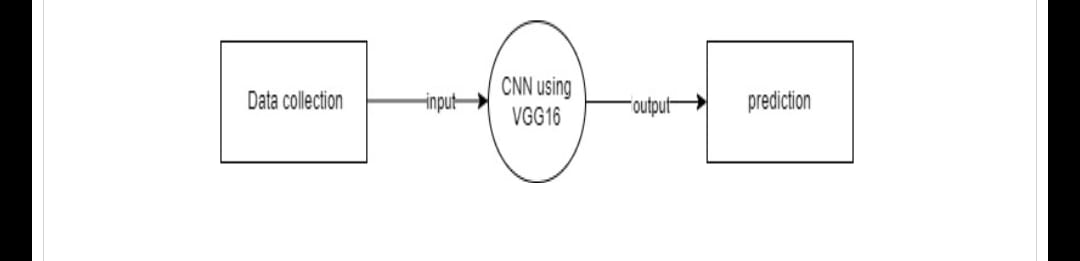
\includegraphics[width=15cm]{ezyzip/img/level1.jpg}
	\caption{\small Data Flow Diagram level - 0 of Table Tech.}
	\label{fig:polarization}
\end{figure}

\nsubsection{Data Flow Diagram}
\begin{figure}[H]
	\centering
	 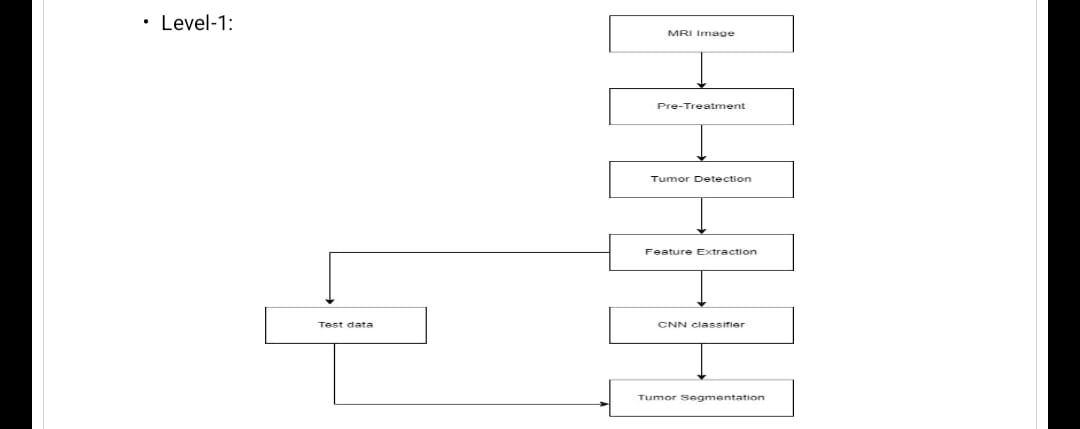
\includegraphics[width=15cm]{ezyzip/img/level2.jpg}
	\caption{\small Data Flow Diagram level - 1 of Table Tech.}
	\label{fig:polarization}
\end{figure}	


\nsubsection{Data Flow Diagram}
\begin{figure}[H]
	\centering
	 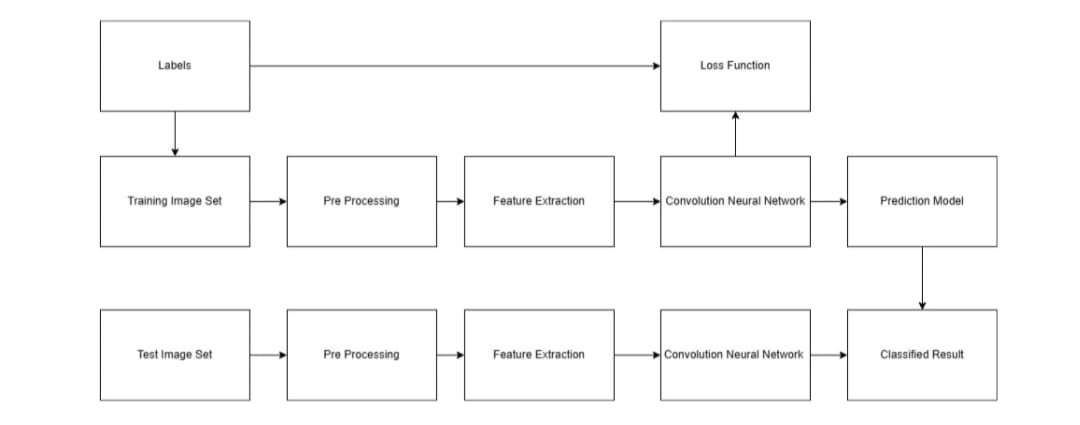
\includegraphics[width=15cm]{ezyzip/img/dataflow.jpg}
	\caption{\small  Data Flow Diagram level - 2 of Table Tech}
	\label{fig:polarization}
\end{figure}	

\nsubsection{Data Flow Diagram}
\begin{figure}[H]
	\centering
	 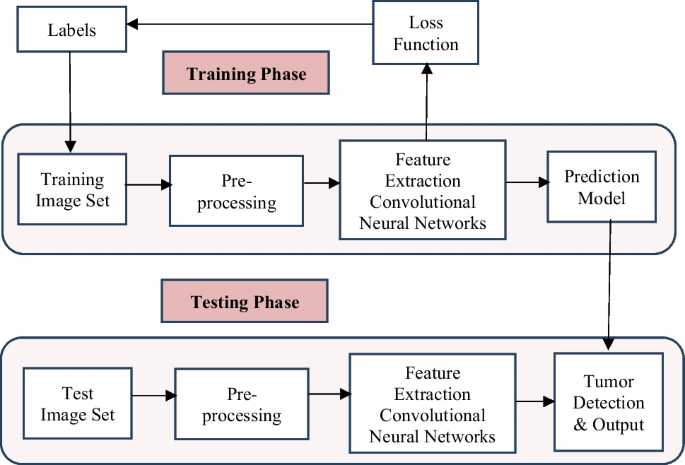
\includegraphics[width=15cm]{ezyzip/img/classdiagrambrain.png}
	\caption{\small class Diagram of Table Tech.}
	\label{fig:polarization}
\end{figure}	
     

\nsubsection{Data Flow Diagram}
\begin{figure}[H]
	\centering
	 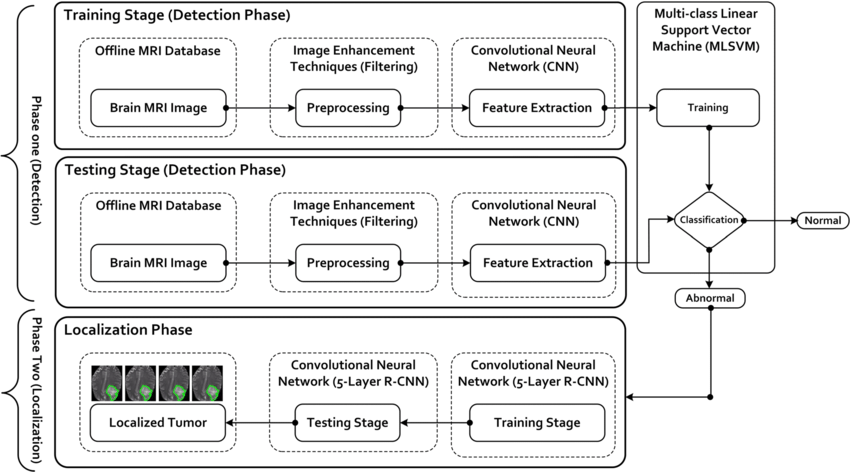
\includegraphics[width=15cm]{ezyzip/img/flowchartbrain.png}
	\caption{\small flow Diagram of Table Tech.}
	\label{fig:polarization}
\end{figure}	
     








